\subsection{Recombination}
In the recombination step, a crossover function is used to pair parents in order to produce a child. This child will belong to the next generation. The model performs a uniform crossover, meaning each gene will be considered separately when pairing the parents \cite{BOOK:GA}. For each song, the notes, chords and rests are considered as the genes of a song. Two parents produce only one child by uniformly selecting genes from one of the two parents. 
On figure \ref{fig:cross_init}, an example of two songs, that are considered as parents, are graphically displayed. During the crossover process, the model iterates over all the genes in both parents and selects only one or the other to pass to the resulting child. Both genes have an equal chance of being selected. On figure \ref{fig:cross_7} a sample child of the corresponding parents is illustrated.
\begin{figure}[H]
    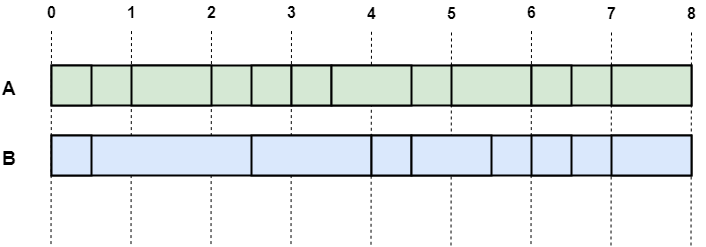
\includegraphics[width=\linewidth]{Fotos/crossover/init.png}
	\caption{Graphical display of two parents A and B. Each rectangle represents a note, chord or rest with their corresponding length. The horizontal axis represents time.}
	\label{fig:cross_init}
\end{figure}
\begin{figure}[H]
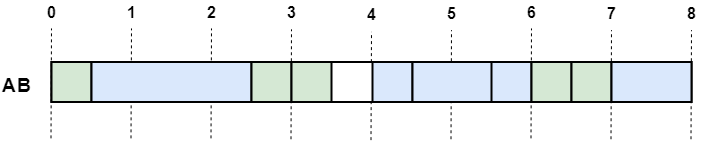
\includegraphics[width=\linewidth]{Fotos/crossover/last.png}
\caption{The child generated from the parents A and B.}
\label{fig:cross_7}
\end{figure}
Notice that there is a gap in the child song at time offset $3.5$. This is the result of selecting parent B's gene at time offset $4$ instead of the corresponding gene of parent A's at time offset $3.5$. 

At each recombination step, all the parents are paired with each other. If there are \(N\) parents, the number of children will be equal to \( \frac{N * (N-1)}{2} \). After the recombination, the fitness of each child will be calculated.